\documentclass[
11pt, % The default document font size, options: 10pt, 11pt, 12pt
%codirector, % Uncomment to add a codirector to the title page
]{charter} 


% El títulos de la memoria, se usa en la carátula y se puede usar el cualquier lugar del documento con el comando \ttitle
\titulo{Análisis de signos vitales mediante técnicas de visión por computadora} 

% Nombre del posgrado, se usa en la carátula y se puede usar el cualquier lugar del documento con el comando \degreename
\posgrado{Carrera de Especialización en Inteligencia Artificial} 
%\posgrado{Carrera de Especialización en Internet de las Cosas} 
%\posgrado{Carrera de Especialización en Inteligencia Artificial}
%\posgrado{Maestría en Sistemas Embebidos} 
%\posgrado{Maestría en Internet de las cosas}

% Tu nombre, se puede usar el cualquier lugar del documento con el comando \authorname
% IMPORTANTE: no omitir titulaciones ni tildación en los nombres, también se recomienda escribir los nombres completos (tal cual los tienen en su documento)
\autor{Ing. Santiago Ruiz}

% El nombre del director y co-director, se puede usar el cualquier lugar del documento con el comando \supname y \cosupname y \pertesupname y \pertecosupname
\director{Esp. Ing. Gerardo Alexis Vilcamiza Espinoza}
\pertenenciaDirector{FIUBA} 
\codirector{} % para que aparezca en la portada se debe descomentar la opción codirector en los parámetros de documentclass
\pertenenciaCoDirector{FIUBA}

% Nombre del cliente, quien va a aprobar los resultados del proyecto, se puede usar con el comando \clientename y \empclientename
\cliente{Médicos de atención remota}
\empresaCliente{Prepagas que ofrecen telemedicina}

\fechaINICIO{24 de agosto de 2026}		%Fecha de inicio de la cursada de GdP \fechaInicioName
\fechaFINALPlan{18 de octubre de 2026} 	%Fecha de final de cursada de GdP
\fechaFINALTrabajo{5 de abril de 2027}	%Fecha de defensa pública del trabajo final


\begin{document}
	
	\maketitle
	\thispagestyle{empty}
	\pagebreak
	
	
	\thispagestyle{empty}
	{\setlength{\parskip}{0pt}
		\tableofcontents{}
	}
	\pagebreak
	
	
	\section*{Registros de cambios}
	\label{sec:registro}
	
	
	\begin{table}[ht]
		\label{tab:registro}
		\centering
		\begin{tabularx}{\linewidth}{@{}|c|X|c|@{}}
			\hline
			\rowcolor[HTML]{C0C0C0} 
			Revisión & \multicolumn{1}{c|}{\cellcolor[HTML]{C0C0C0}Detalles de los cambios realizados} & Fecha      \\ \hline
			0      & Creación del documento                                 &\fechaInicioName \\ \hline
			1      & Se completa hasta el punto 5 inclusive                 & 6 de septiembre de 2026 \\ \hline
			2      & Se completa hasta el punto 9 inclusive                 & 13 de septiembre de 2026 \\ \hline
			%		  Se puede agregar algo más \newline
			%		  En distintas líneas \newline
			%		  Así                                                    & {día} de {mes} de 202X \\ \hline
			%3      & Se completa hasta el punto 12 inclusive                & {día} de {mes} de 202X \\ \hline
			%4      & Se completa el plan	                                 & {día} de {mes} de 202X \\ \hline
			
			% Si hay más correcciones pasada la versión 4 también se deben especificar acá
			
		\end{tabularx}
	\end{table}
	
	\pagebreak
	
	
	
	\section*{Acta de constitución del proyecto}
	\label{sec:acta}
	
	\begin{flushright}
		Buenos Aires, \fechaInicioName
	\end{flushright}
	
	\vspace{2cm}
	
	Por medio de la presente se acuerda con el \authorname\hspace{1px} que su Trabajo Final de la \degreename\hspace{1px} se titulará ``\ttitle'' y consistirá en {la implementación de un sistema basado en técnicas de fotopletismografía remota (rPPG) capaz de estimar, de manera no invasiva, signos vitales de una persona como la frecuencia cardíaca}. El trabajo tendrá un presupuesto preliminar estimado de {600} horas y un costo estimado de \textcolor{red}{\$ XXX}, con fecha de inicio el \fechaInicioName\hspace{1px} y fecha de presentación pública el \fechaFinalName.
	
	Se adjunta a esta acta la planificación inicial.
	
	\vfill
	
	% Esta parte se construye sola con la información que hayan cargado en el preámbulo del documento y no debe modificarla
	\begin{table}[ht]
		\centering
		\begin{tabular}{ccc}
			\begin{tabular}[c]{@{}c@{}}Dr. Ing. Ariel Lutenberg \\ Director posgrado FIUBA\end{tabular} & \hspace{2cm} & \begin{tabular}[c]{@{}c@{}}\clientename \\ \empclientename \end{tabular} \vspace{2.5cm} \\ 
			\multicolumn{3}{c}{\begin{tabular}[c]{@{}c@{}} \supname \\ Director del Trabajo Final\end{tabular}} \vspace{2.5cm} \\
		\end{tabular}
	\end{table}
	
	
	
	
	\section{1. Descripción técnica-conceptual del proyecto a realizar}
	\label{sec:descripcion}
	
	El monitoreo de signos vitales constituye una fuente de información fundamental para evaluar el estado de salud y bienestar de una persona. Entre estos signos, se encuentran la frecuencia cardíaca y la frecuencia respiratoria. Tradicionalmente, esta medición requiere sensores en contacto directo con la piel (electrodos, oxímetros de dedo, bandas pectorales), lo que limita su uso en escenarios en que el contacto físico es incómodo, poco práctico o directamente imposible. Un ejemplo de esta situación es una consulta de telemedicina, en la que el profesional de la salud no tiene contacto físico con su paciente y, por lo tanto, no puede recurrir al instrumental habitual de un consultorio presencial.
	
	En los últimos años, la fotopletismografía remota (\textit{remote photoplethysmography}, rPPG) surgió como una alternativa \textit{contactless} que permite estimar signos vitales a partir de video. Esta técnica aprovecha las variaciones sutiles e imperceptibles al ojo humano en el color de la piel que produce el flujo sanguíneo sincronizado con el ciclo cardíaco. Los primeros trabajos en esta línea utilizaban técnicas clásicas de procesamiento de señales (separación ciega de fuentes, filtrado de color) para extraer esta información a partir de video facial. El avance del \textit{deep learning} aplicado a visión por computadora amplió significativamente la robustez de estas técnicas frente a los métodos clásicos, con arquitecturas como DeepPhys (redes convolucionales con mecanismos de atención) o PhysNet (redes 3D espacio-temporales). A pesar de estos avances, todavía persisten desafíos relevantes: artefactos de movimiento, variaciones de iluminación, diferencias en el tono de piel y una brecha de rendimiento entre condiciones controladas de laboratorio y escenarios de uso reales.
	
	Este proyecto surge como un trabajo individual de carácter exploratorio y aplicado, sin financiamiento externo ni acuerdos de confidencialidad asociados. La propuesta de valor del proyecto consiste en ofrecer una alternativa de bajo costo y sin fricción para obtener una estimación de signos vitales durante una consulta remota, dado que solo requiere una cámara. Esto habitualmente ya se encuentra disponible en el dispositivo que el paciente utiliza para acceder a la consulta. Se distingue de las soluciones basadas en sensores de contacto, que dependen de instrumental específico y no siempre está disponible fuera de un entorno clínico. El principal interesado en este tipo de solución es el profesional de la salud que realiza consultas de telemedicina, así como las plataformas que dan soporte a esta modalidad de atención, quienes valoran contar con información objetiva del paciente.
	
	El proyecto se encuentra en una etapa de prueba de concepto. En esta, se busca validar la viabilidad técnica de estimar la frecuencia cardíaca a partir de video, y a partir de esa misma señal, obtener una estimación de la frecuencia respiratoria. Para ello, se comparará el desempeño de un enfoque clásico y uno basado en \textit{deep learning} sobre datasets públicos reconocidos en la literatura de rPPG. Estos enfoques serán contrastados con mediciones de referencia obtenidas con sensores de contacto.
	
	La solución propuesta toma como entrada un video del rostro de la persona capturado con una cámara convencional, y produce como salida una estimación numérica de la frecuencia cardíaca y respiratoria, que pueden contrastarse contra una medición de referencia. En la figura \ref{fig:diagBloques} se presenta el diagrama en bloques del sistema. Se observa que, en primer lugar, se realiza la detección facial y la selección de una región de interés (ROI) sobre el video de entrada. Luego, se extrae una única señal fisiológica (rPPG), ya sea mediante un pipeline clásico de procesamiento de imagen o mediante un modelo de \textit{deep learning} de tipo espacio-temporal. A continuación, dicha señal se filtra en dos bandas de frecuencia distintas, a partir de las que se estiman la frecuencia cardíaca y la frecuencia respiratoria (mediante análisis espectral o directamente a la salida del modelo). Finalmente, los valores estimados se comparan contra las mediciones de los sensores de referencia a los fines de validar el desempeño del sistema.
	
	\begin{figure}[htpb]
		\centering 
		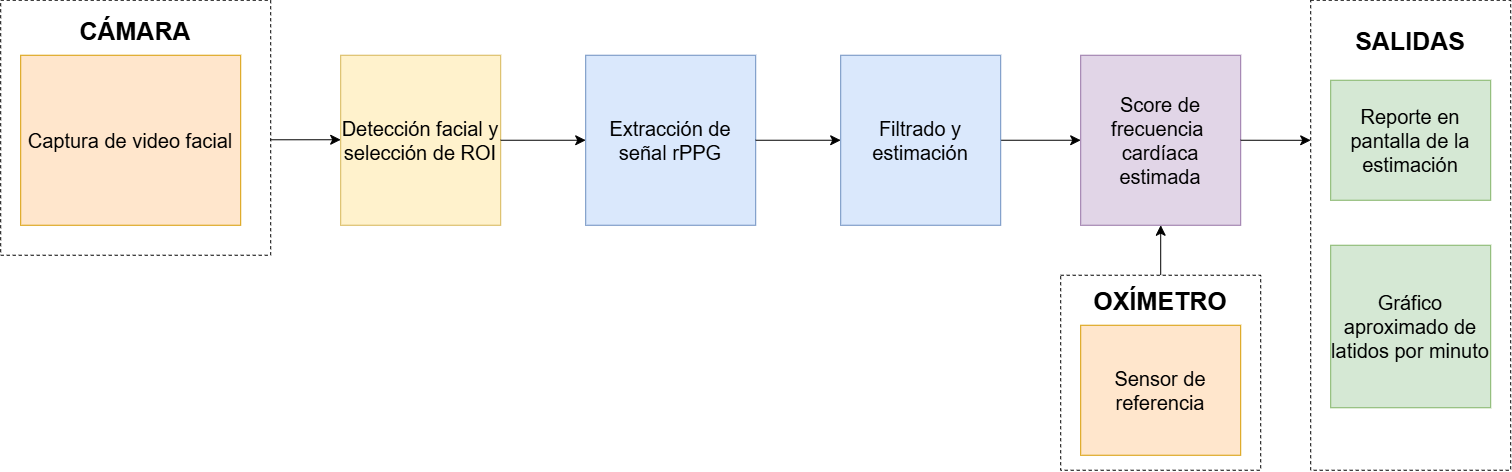
\includegraphics[width=.85\textwidth]{./Figuras/diagBloques.png}
		\caption{Diagrama en bloques del sistema.}
		\label{fig:diagBloques}
	\end{figure}
	
	\section{2. Identificación y análisis de los interesados}
	\label{sec:interesados}
	
	\begin{table}[ht]
		%\caption{Identificación de los interesados}
		%\label{tab:interesados}
		\begin{tabularx}{\linewidth}{@{}|l|X|X|l|@{}}
			\hline
			\rowcolor[HTML]{C0C0C0} 
			Rol           & Nombre y Apellido & Organización 	& Puesto 	\\ \hline
			Cliente       & \clientename      &\empclientename	& -      	\\ \hline
			Responsable   & \authorname       & FIUBA        	& Alumno 	\\ \hline
			Orientador    & \supname	      & \pertesupname 	& Director del Trabajo Final \\ \hline
			Usuario final & -                 & Prepagas/Pacientes & Profesionales/Pacientes  \\ \hline
		\end{tabularx}
	\end{table}
	
	A continuación se listan las principales características de cada interesado:
	
	\begin{itemize}
		\item Cliente: valora contar con información objetiva y no invasiva del estado fisiológico del paciente durante una consulta remota, en un contexto donde hoy no dispone de instrumental de medición.
		\item Orientador: colabora en la definición del alcance técnico del proyecto y en la validación de las decisiones metodológicas relacionadas con las técnicas de visión por computadora y \textit{deep learning} aplicadas.
		\item Usuario final: el profesional de la salud valora la rapidez y la no invasividad de la medición, mientras que el paciente valora no depender de instrumental adicional ni de conocimientos técnicos para su uso.
	\end{itemize}
	
	\section{3. Propósito del proyecto}
	\label{sec:proposito}
	
	El propósito de este proyecto es diseñar, implementar y evaluar un sistema basado en visión por computadora y \textit{deep learning} capaz de estimar, de manera no invasiva y a partir de video facial, la frecuencia cardíaca y respiratoria de una persona. Se busca comparar su desempeño frente a mediciones de referencia obtenidas con sensores de contacto, de modo de sentar una base técnica que permita, en un futuro, incorporar esta capacidad a escenarios de telemedicina u otros contextos en los que la medición por contacto resulte poco práctica.
	
	\section{4. Alcance del proyecto}
	\label{sec:alcance}
	
	El proyecto incluye:
	\begin{itemize}
		\item Relevamiento del estado del arte en fotopletismografía remota (rPPG), desde métodos clásicos hasta enfoques basados en \textit{deep learning}.
		\item Implementación de un pipeline clásico (\textit{baseline}) de extracción de señal rPPG: detección facial, selección de región de interés (ROI), extracción de señal de color, filtrado y estimación de la frecuencia cardíaca mediante análisis espectral.
		\item Implementación o adaptación de un modelo de \textit{deep learning} (arquitectura de tipo CNN espacio-temporal) para la estimación de la frecuencia cardíaca a partir de video.
		\item Entrenamiento y validación del modelo utilizando datasets públicos reconocidos en la literatura de rPPG (UBFC-rPPG como dataset principal, PURE como dataset complementario).
		\item Comparación del desempeño del pipeline clásico y del modelo de \textit{deep learning}, utilizando métricas estándar (error absoluto medio, raíz del error cuadrático medio, coeficiente de correlación de Pearson).
		\item Documentación de resultados, limitaciones del sistema y condiciones de uso válidas.
	\end{itemize}
	
	El presente proyecto no incluye:
	\begin{itemize}
		\item La estimación de otras variables fisiológicas de mayor complejidad, como la presión arterial o la saturación de oxígeno (SpO2).
		\item El desarrollo de una interfaz de usuario o de una integración con una plataforma de telemedicina real.
		\item La validación clínica del sistema con pacientes reales ni la obtención de aprobaciones regulatorias para su uso como dispositivo médico.
		\item El despliegue del sistema en un entorno de producción o su optimización para ejecución en tiempo real sobre hardware embebido.
	\end{itemize}
	
	\section{5. Supuestos del proyecto}
	\label{sec:supuestos}
	
	Para el desarrollo del presente proyecto se supone que:
	
	\begin{itemize}
		\item Los datasets públicos a utilizar (UBFC-rPPG, PURE) se encuentran disponibles y accesibles durante todo el desarrollo del proyecto.
		\item Se cuenta con el tiempo y los recursos de cómputo necesarios (incluyendo, de ser necesario, acceso a GPU) para entrenar y evaluar los modelos de \textit{deep learning} propuestos.
		\item Las condiciones de captura de video consideradas (iluminación razonablemente estable, rostro visible y sin oclusiones significativas) son representativas de un escenario típico de videollamada o consulta de telemedicina.
		\item El alcance del proyecto se limita a una prueba de concepto técnica, por lo que no se requiere validación clínica ni cumplimiento de normativa sanitaria para su desarrollo.
	\end{itemize}
	
	
	\section{6. Requerimientos}
	\label{sec:requerimientos}
	
	Los requerimientos se agrupan en cinco categorías: funcionales, de desempeño, de datos y validación, de documentación, y regulatorios/éticos.
	
	\begin{enumerate}
		\item Requerimientos funcionales
		\begin{enumerate}
			\item El sistema debe detectar el rostro de la persona en al menos el 95\% de los \textit{frames} de un video con iluminación estable. (Prioridad: alta)
			\item El sistema debe extraer una señal fisiológica (rPPG) a partir de la región de interés (ROI) facial detectada. (Prioridad: alta)
			\item El sistema debe estimar la frecuencia cardíaca (HR) del sujeto, expresada en latidos por minuto (bpm). (Prioridad: alta)
			\item El sistema debe estimar la frecuencia respiratoria (RR) del sujeto, expresada en respiraciones por minuto, a partir de la misma señal utilizada para estimar la HR. (Prioridad: alta)
			\item El sistema debe implementar un \textit{pipeline} clásico de estimación (sin \textit{deep learning}) como línea base de comparación. (Prioridad: alta)
			\item El sistema debe implementar al menos un modelo de \textit{deep learning} de tipo espacio-temporal para la estimación de la HR. (Prioridad: alta)
			\item El sistema debe poder procesar, en modo \textit{offline}, videos provenientes de los datasets públicos seleccionados. (Prioridad: alta)
			\item El sistema podrá, de forma opcional, procesar video capturado en vivo desde una cámara web con fines exploratorios. (Prioridad: baja, opcional)
		\end{enumerate}
		\item Requerimientos de desempeño
		\begin{enumerate}
			\item La estimación de HR, tanto del \textit{pipeline} clásico como del modelo de \textit{deep learning}, debe alcanzar un error absoluto medio (MAE) no mayor a 5 bpm sobre el dataset UBFC-rPPG. (Prioridad: alta)
			\item El coeficiente de correlación de Pearson entre la HR estimada y la HR de referencia debe ser mayor a 0,8 sobre el dataset UBFC-rPPG. (Prioridad: media)
			\item El tiempo de procesamiento de un video de un minuto de duración, en modo \textit{offline}, no debe superar los dos minutos sobre el hardware disponible para el proyecto. (Prioridad: baja)
		\end{enumerate}
		\item Requerimientos de datos y validación
		\begin{enumerate}
			\item El sistema debe evaluarse, como mínimo, sobre el dataset UBFC-rPPG. (Prioridad: alta)
			\item De contar con tiempo suficiente, el sistema debe evaluarse adicionalmente sobre el dataset PURE. (Prioridad: media, opcional)
			\item El conjunto de datos utilizado para entrenamiento y el de evaluación deben mantenerse disjuntos, sin superposición de sujetos. (Prioridad: alta)
		\end{enumerate}
		\item Requerimientos de documentación
		\begin{enumerate}
			\item Se debe documentar la arquitectura del \textit{pipeline} clásico y del modelo de \textit{deep learning} utilizados. (Prioridad: alta)
			\item Se deben documentar las métricas obtenidas y las condiciones bajo las cuales se obtuvieron. (Prioridad: alta)
			\item Se deben documentar las limitaciones identificadas del sistema y sus condiciones de uso válidas. (Prioridad: media)
		\end{enumerate}
		\item Requerimientos regulatorios y éticos
		\begin{enumerate}
			\item El proyecto debe utilizar exclusivamente datasets públicos que cuenten con consentimiento informado de los sujetos y licencia de uso académico o de investigación. (Prioridad: alta)
			\item El sistema no debe presentarse ni utilizarse como un dispositivo médico certificado, dado que no cuenta con validación clínica ni aprobación regulatoria. (Prioridad: alta)
		\end{enumerate}
	\end{enumerate}
	
	\section{7. Historias de usuarios (\textit{Product backlog})}
	\label{sec:backlog}
	
Los \textit{story points} de cada historia se calculan como la suma de tres subpuntajes, cada uno en una escala de 1 a 5: complejidad, dificultad e incertidumbre.

	\begin{enumerate}
		\item ``Como investigador, quiero implementar la detección facial y la selección de la región de interés (ROI) sobre un video, para poder aislar la zona de piel relevante para la estimación de la señal fisiológica."
		
		\textit{Story points}: 5 (complejidad: 2, dificultad: 2, incertidumbre: 1)
		
		\item ``Como investigador, quiero extraer la señal rPPG mediante un \textit{pipeline} clásico de procesamiento de imagen, para contar con una línea base de comparación."
		
		\textit{Story points}: 8 (complejidad: 3, dificultad: 3, incertidumbre: 2)
		
		\item ``Como investigador, quiero estimar la frecuencia cardíaca a partir de la señal rPPG mediante análisis espectral, para validar la viabilidad del enfoque clásico."
		
		\textit{Story points}: 5 (complejidad: 2, dificultad: 2, incertidumbre: 1)
		
		\item ``Como investigador, quiero estimar la frecuencia respiratoria a partir de la misma señal rPPG utilizada para la frecuencia cardíaca, para evaluar la viabilidad de obtener ambas variables sin duplicar el \textit{pipeline} de captura."
		
		\textit{Story points}: 5 (complejidad: 2, dificultad: 1, incertidumbre: 2)
		
		\item ``Como investigador, quiero implementar o adaptar un modelo de \textit{deep learning} de tipo espacio-temporal, para estimar la frecuencia cardíaca directamente a partir del video."
		
		\textit{Story points}: 13 (complejidad: 5, dificultad: 4, incertidumbre: 4)
		
		\item ``Como investigador, quiero entrenar el modelo de \textit{deep learning} sobre el dataset UBFC-rPPG, para contar con un modelo ajustado a datos reales de referencia."
		
		\textit{Story points}: 8 (complejidad: 3, dificultad: 3, incertidumbre: 2)
		
		\item ``Como investigador, quiero calcular las métricas de error (MAE, RMSE, correlación de Pearson) entre las estimaciones y las mediciones de referencia, para poder comparar objetivamente ambos enfoques."
		
		\textit{Story points}: 5 (complejidad: 2, dificultad: 2, incertidumbre: 1)
		
		\item ``Como investigador, quiero documentar los resultados obtenidos y las limitaciones identificadas, para dejar registro de las condiciones de uso válidas del sistema."
		
		\textit{Story points}: 3 (complejidad: 1, dificultad: 1, incertidumbre: 1)
		
		\item ``Como profesional de la salud, quiero que el sistema entregue una estimación numérica clara de la frecuencia cardíaca y respiratoria, para poder interpretarla rápidamente en una demostración del sistema."
		
		\textit{Story points}: 5 (complejidad: 2, dificultad: 2, incertidumbre: 1)
	\end{enumerate}
	
	\section{8. Entregables principales del proyecto}
	\label{sec:entregables}
	
	Los entregables del proyecto son:
	
	\begin{itemize}
		\item Código fuente del \textit{pipeline} clásico de estimación de frecuencia cardíaca y respiratoria.
		\item Código fuente y pesos entrenados del modelo de \textit{deep learning}.
		\item Script de evaluación y comparación de métricas (MAE, RMSE, correlación de Pearson) entre ambos enfoques.
		\item Reporte de resultados, con las limitaciones identificadas y las condiciones de uso válidas del sistema.
		\item Memoria del trabajo final.
		\item Presentación para la defensa pública del trabajo.
	\end{itemize}
	
	\section{9. Desglose del trabajo en tareas}
	\label{sec:wbs}
	
	\begin{enumerate}
		\item Relevamiento y diseño (60 h)
		\begin{enumerate}
			\item Revisión del estado del arte en rPPG (20 h)
			\item Selección y descarga de datasets públicos (10 h)
			\item Definición de la arquitectura del \textit{pipeline} clásico y del modelo de \textit{deep learning} (20 h)
			\item Definición de las métricas de evaluación (10 h)
		\end{enumerate}
		\item Implementación del \textit{pipeline} clásico (120 h)
		\begin{enumerate}
			\item Implementación de la detección facial y selección de ROI (30 h)
			\item Implementación de la extracción de la señal rPPG (30 h)
			\item Implementación del filtrado y la estimación espectral de la HR (30 h)
			\item Implementación del filtrado y la estimación espectral de la RR (30 h)
		\end{enumerate}
		\item Implementación y entrenamiento del modelo de \textit{deep learning} (180 h)
		\begin{enumerate}
			\item Preprocesamiento de datos para el entrenamiento (30 h)
			\item Implementación de la arquitectura del modelo (40 h)
			\item Entrenamiento del modelo (40 h)
			\item Ajuste de hiperparámetros (40 h)
			\item Validación del modelo sobre el conjunto de test (30 h)
		\end{enumerate}
		\item Evaluación y comparación de enfoques (100 h)
		\begin{enumerate}
			\item Cálculo de métricas de error (MAE, RMSE) (30 h)
			\item Cálculo del coeficiente de correlación de Pearson (20 h)
			\item Análisis comparativo entre el \textit{pipeline} clásico y el modelo de \textit{deep learning} (30 h)
			\item Identificación de limitaciones y condiciones de uso válidas (20 h)
		\end{enumerate}
		\item Documentación y cierre (140 h)
		\begin{enumerate}
			\item Redacción de la primera versión de la memoria del trabajo final (30 h)
			\item Revisión y correcciones sugeridas por el director (40 h)
			\item Redacción de la versión final de la memoria (30 h)
			\item Preparación de la presentación para la defensa pública (20 h)
			\item Ensayo de la defensa pública (20 h)
		\end{enumerate}
	\end{enumerate}
	
	Cantidad total de horas: 600 h.
	
	\section{10. Diagrama de Activity On Node}
	\label{sec:AoN}
	
	\begin{consigna}{red}
		Armar el AoN a partir del WBS definido en la etapa anterior.
		
		Una herramienta simple para desarrollar los diagramas es el Draw.io (\url{https://app.diagrams.net/}).
		\href{https://app.diagrams.net}{Draw.io}
		
		
		\begin{figure}[htpb]
			\centering 
			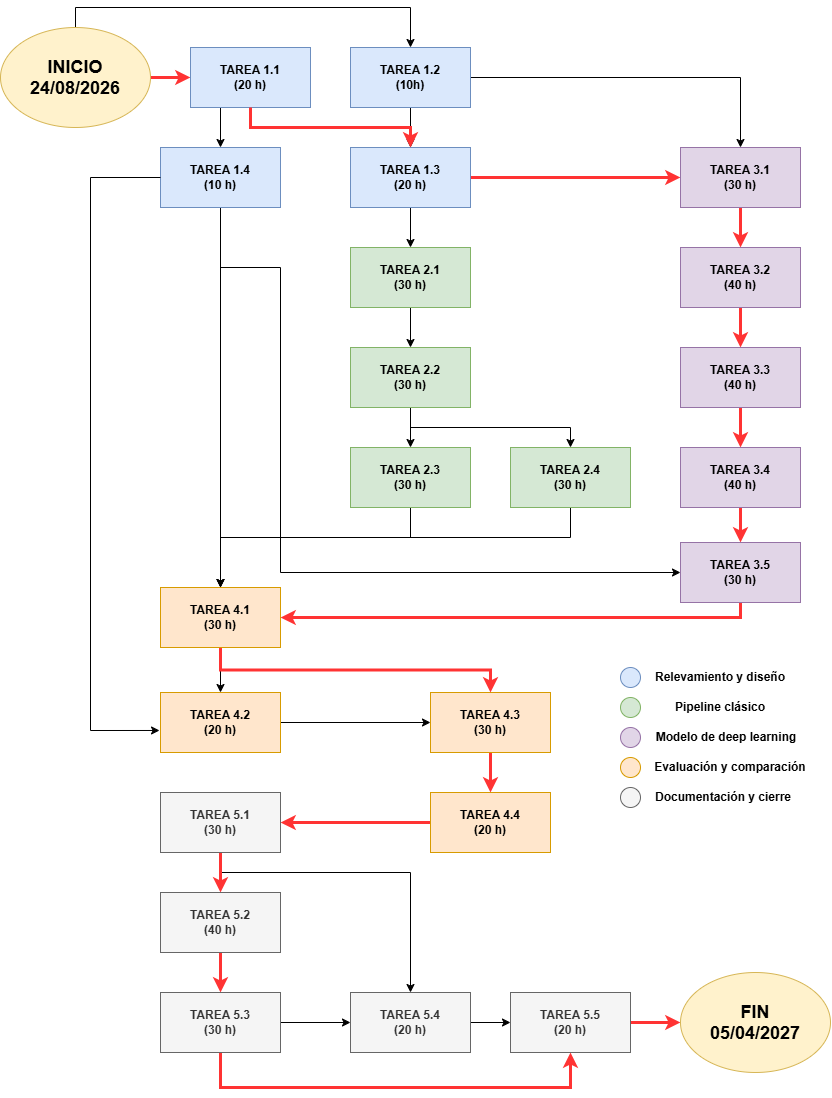
\includegraphics[width=.8\textwidth]{./Figuras/AoN.png}
			\caption{Diagrama de \textit{Activity on Node}.}
			\label{fig:AoN}
		\end{figure}
		
		Indicar claramente en qué unidades están expresados los tiempos.
		De ser necesario indicar los caminos semi críticos y analizar sus tiempos mediante un cuadro.
		Es recomendable usar colores y un cuadro indicativo describiendo qué representa cada color.
		
	\end{consigna}
	
	\section{11. Diagrama de Gantt}
	\label{sec:gantt}
	
	\begin{consigna}{red}
		Existen muchos programas y recursos \textit{online} para hacer diagramas de Gantt, entre los cuales destacamos:
		
		\begin{itemize}
			\item Planner
			\item GanttProject
			\item Trello + \textit{plugins}. En el siguiente link hay un tutorial oficial: \\ \url{https://blog.trello.com/es/diagrama-de-gantt-de-un-proyecto}
			\item Creately, herramienta online colaborativa. \\\url{https://creately.com/diagram/example/ieb3p3ml/LaTeX}
			\item Se puede hacer en latex con el paquete \textit{pgfgantt}\\ \url{http://ctan.dcc.uchile.cl/graphics/pgf/contrib/pgfgantt/pgfgantt.pdf}
		\end{itemize}
		
		Pegar acá una captura de pantalla del diagrama de Gantt, cuidando que la letra sea suficientemente grande como para ser legible. 
		Si el diagrama queda demasiado ancho, se puede pegar primero la ``tabla'' del Gantt y luego pegar la parte del diagrama de barras del diagrama de Gantt.
		
		Configurar el software para que en la parte de la tabla muestre los códigos del EDT (WBS).\\
		Configurar el software para que al lado de cada barra muestre el nombre de cada tarea.\\
		Revisar que la fecha de finalización coincida con lo indicado en el Acta Constitutiva.
		
		En la figura \ref{fig:gantt}, se muestra un ejemplo de diagrama de gantt realizado con el paquete de \textit{pgfgantt}. 
		En la plantilla pueden ver el código que lo genera y usarlo de base para construir el propio.
		
		Las fechas pueden ser calculadas utilizando alguna de las herramientas antes citadas. Sin embargo, el siguiente ejemplo
		fue elaborado utilizando 
		\href{https://docs.google.com/spreadsheets/d/1fBz8NhSpc4tkkhz3KjJCbh1nR_ltDkfEcZi4tZXduqs}{esta hoja de cálculo}.
		
		Es importante destacar que el ancho del diagrama estará dado por la longitud del texto utilizado para las tareas 
		(Ejemplo: tarea 1, tarea 2, etcétera) y el valor \textit{x unit}. Para mejorar la apariencia del diagrama, es necesario
		ajustar este valor y, quizás, acortar los nombres de las tareas.
		
		\begin{figure}[htpb]
			\begin{center}
				\begin{ganttchart}[
					time slot unit=day,
					time slot format=isodate,
					x unit=0.038cm,
					y unit title=0.7cm,
					y unit chart=0.6cm,
					milestone/.append style={xscale=4}
					]{2021-03-05}{2021-12-16}
					\gantttitlecalendar*{2021-03-05}{2021-12-16}{year} \\
					\gantttitlecalendar*{2021-03-05}{2021-12-16}{month} \\
					\ganttgroup{Duración Total}{2021-03-05}{2021-12-16} \\
					%%%%%%%%%%%%%%%%%Organización
					\ganttgroup{Organización}{2021-03-05}{2021-04-16} \\
					\ganttbar{Planificación del proyecto}{2021-03-05}{2021-04-15} \\
					%%%%%%%%%%%%%%%%%Ejecución
					\ganttgroup{Ejecución}{2021-04-16}{2021-10-21} \\
					\ganttbar{Tarea 1}{2021-04-16}{2021-04-29} \\
					\ganttbar{Tarea 2}{2021-04-30}{2021-05-13} \\
					\ganttbar{Tarea 3}{2021-05-14}{2021-05-27} \\
					\ganttbar{Tarea 4}{2021-05-28}{2021-07-12} \\
					\ganttbar{Tarea 5}{2021-07-13}{2021-08-09} \\
					\ganttbar{Tarea 6}{2021-08-10}{2021-09-23} \\
					\ganttbar{Tarea 7}{2021-09-24}{2021-09-30} \\
					\ganttbar{Tarea 8}{2021-10-01}{2021-10-14} \\
					\ganttbar{Tarea 9}{2021-10-15}{2021-10-21} \\
					% %%%%%%%%%%%%%%%%%Finalización
					\ganttgroup{Finalización}{2021-10-22}{2021-12-16} \\
					\ganttbar{Memoria v1}{2021-10-22}{2021-11-04} \\
					\ganttbar{Memoria v2}{2021-11-05}{2021-11-18} \\
					\ganttbar{Memoria final}{2021-11-19}{2021-12-02} \\
					% La fecha del siguiente milestone es la fecha en que terminamos la memoria
					\ganttmilestone{Enviar memoria al director}{2021-12-02} \\
					\ganttbar{Elaborar la presentación}{2021-12-03}{2021-12-16} \\
					\ganttmilestone{Ensayo de la presentación}{2021-12-16} \\
					%%%%%%%%%%%%%%%%%%%%%%%%%%%%%%%%%%%%%%%%%%%%%%%%%%%%%%%%%%%%%%%
				\end{ganttchart}
			\end{center}
			\caption{Diagrama de gantt de ejemplo}
			\label{fig:gantt}
		\end{figure}
		
		
		\begin{landscape}
			\begin{figure}[htpb]
				\centering 
				\includegraphics[height=.85\textheight]{./Figuras/Gantt-2.png}
				\caption{Ejemplo de diagrama de Gantt (apaisado).} %Modificar este título acorde.
				\label{fig:diagGantt}
			\end{figure}
			
		\end{landscape}
		
	\end{consigna}
	
	
	\section{12. Presupuesto detallado del proyecto}
	\label{sec:presupuesto}
	
	\begin{consigna}{red}
		Si el proyecto es complejo entonces separarlo en partes:
		\begin{itemize}
			\item Un total global, indicando el subtotal acumulado por cada una de las áreas.
			\item El desglose detallado del subtotal de cada una de las áreas.
		\end{itemize}
		
		IMPORTANTE: No olvidarse de considerar los COSTOS INDIRECTOS.
		
		Incluir la aclaración de si se emplea como moneda el peso argentino (ARS) o si se usa moneda extranjera (USD, EUR, etc). Si es en moneda extranjera se debe indicar la tasa de conversión respecto a la moneda local en una fecha dada.
		
	\end{consigna}
	
	\begin{table}[htpb]
		\centering
		\begin{tabularx}{\linewidth}{@{}|X|c|r|r|@{}}
			\hline
			\rowcolor[HTML]{C0C0C0} 
			\multicolumn{4}{|c|}{\cellcolor[HTML]{C0C0C0}COSTOS DIRECTOS} \\ \hline
			\rowcolor[HTML]{C0C0C0} 
			Descripción &
			\multicolumn{1}{c|}{\cellcolor[HTML]{C0C0C0}Cantidad} &
			\multicolumn{1}{c|}{\cellcolor[HTML]{C0C0C0}Valor unitario} &
			\multicolumn{1}{c|}{\cellcolor[HTML]{C0C0C0}Valor total} \\ \hline
			&
			\multicolumn{1}{c|}{} &
			\multicolumn{1}{c|}{} &
			\multicolumn{1}{c|}{} \\ \hline
			&
			\multicolumn{1}{c|}{} &
			\multicolumn{1}{c|}{} &
			\multicolumn{1}{c|}{} \\ \hline
			\multicolumn{1}{|l|}{} &
			&
			&
			\\ \hline
			\multicolumn{1}{|l|}{} &
			&
			&
			\\ \hline
			\multicolumn{3}{|c|}{SUBTOTAL} &
			\multicolumn{1}{c|}{} \\ \hline
			\rowcolor[HTML]{C0C0C0} 
			\multicolumn{4}{|c|}{\cellcolor[HTML]{C0C0C0}COSTOS INDIRECTOS} \\ \hline
			\rowcolor[HTML]{C0C0C0} 
			Descripción &
			\multicolumn{1}{c|}{\cellcolor[HTML]{C0C0C0}Cantidad} &
			\multicolumn{1}{c|}{\cellcolor[HTML]{C0C0C0}Valor unitario} &
			\multicolumn{1}{c|}{\cellcolor[HTML]{C0C0C0}Valor total} \\ \hline
			\multicolumn{1}{|l|}{} &
			&
			&
			\\ \hline
			\multicolumn{1}{|l|}{} &
			&
			&
			\\ \hline
			\multicolumn{1}{|l|}{} &
			&
			&
			\\ \hline
			\multicolumn{3}{|c|}{SUBTOTAL} &
			\multicolumn{1}{c|}{} \\ \hline
			\rowcolor[HTML]{C0C0C0}
			\multicolumn{3}{|c|}{TOTAL} &
			\\ \hline
		\end{tabularx}%
	\end{table}
	
	
	\section{13. Gestión de riesgos}
	\label{sec:riesgos}
	
	\begin{consigna}{red}
		a) Identificación de los riesgos (al menos cinco) y estimación de sus consecuencias:
		
		Riesgo 1: detallar el riesgo (riesgo es algo que si ocurre altera los planes previstos de forma negativa)
		\begin{itemize}
			\item Severidad (S): mientras más severo, más alto es el número (usar números del 1 al 10).\\
			Justificar el motivo por el cual se asigna determinado número de severidad (S).
			\item Probabilidad de ocurrencia (O): mientras más probable, más alto es el número (usar del 1 al 10).\\
			Justificar el motivo por el cual se asigna determinado número de (O). 
		\end{itemize}   
		
		Riesgo 2:
		\begin{itemize}
			\item Severidad (S): X.\\
			Justificación...
			\item Ocurrencia (O): Y.\\
			Justificación...
		\end{itemize}
		
		Riesgo 3:
		\begin{itemize}
			\item Severidad (S):  X.\\
			Justificación...
			\item Ocurrencia (O): Y.\\
			Justificación...
		\end{itemize}
		
		
		b) Tabla de gestión de riesgos:      (El RPN se calcula como RPN=SxO)
		
		\begin{table}[htpb]
			\centering
			\begin{tabularx}{\linewidth}{@{}|X|c|c|c|c|c|c|@{}}
				\hline
				\rowcolor[HTML]{C0C0C0} 
				Riesgo & S & O & RPN & S* & O* & RPN* \\ \hline
				&   &   &     &    &    &      \\ \hline
				&   &   &     &    &    &      \\ \hline
				&   &   &     &    &    &      \\ \hline
				&   &   &     &    &    &      \\ \hline
				&   &   &     &    &    &      \\ \hline
			\end{tabularx}%
		\end{table}
		
		Criterio adoptado: 
		
		Se tomarán medidas de mitigación en los riesgos cuyos números de RPN sean mayores a...
		
		Nota: los valores marcados con (*) en la tabla corresponden luego de haber aplicado la mitigación.
		
		c) Plan de mitigación de los riesgos que originalmente excedían el RPN máximo establecido:
		
		Riesgo 1: plan de mitigación (si por el RPN fuera necesario elaborar un plan de mitigación).
		Nueva asignación de S y O, con su respectiva justificación:
		\begin{itemize}
			\item Severidad (S*): mientras más severo, más alto es el número (usar números del 1 al 10).
			Justificar el motivo por el cual se asigna determinado número de severidad (S).
			\item Probabilidad de ocurrencia (O*): mientras más probable, más alto es el número (usar del 1 al 10).
			Justificar el motivo por el cual se asigna determinado número de (O).
		\end{itemize}
		
		Riesgo 2: plan de mitigación (si por el RPN fuera necesario elaborar un plan de mitigación).
		
		Riesgo 3: plan de mitigación (si por el RPN fuera necesario elaborar un plan de mitigación).
		
	\end{consigna}
	
	
	\section{14. Gestión de la calidad}
	\label{sec:calidad}
	
	\begin{consigna}{red}
		Elija al menos diez requerimientos que a su criterio sean los más importantes/críticos/que aportan más valor y para cada uno de ellos indique las acciones de verificación y validación que permitan asegurar su cumplimiento.
		
		\begin{itemize} 
			\item Req \#1: copiar acá el requerimiento con su correspondiente número.
			
			\begin{itemize}
				\item Verificación para confirmar si se cumplió con lo requerido antes de mostrar el sistema al cliente. Detallar.
				\item Validación con el cliente para confirmar que está de acuerdo en que se cumplió con lo requerido. Detallar. 
			\end{itemize}
			
		\end{itemize}
		
		Tener en cuenta que en este contexto se pueden mencionar simulaciones, cálculos, revisión de hojas de datos, consulta con expertos, mediciones, etc.  
		
		Las acciones de verificación suelen considerar al entregable como ``caja blanca'', es decir se conoce en profundidad su funcionamiento interno.  
		
		En cambio, las acciones de validación suelen considerar al entregable como ``caja negra'', es decir, que no se conocen los detalles de su funcionamiento interno.
		
	\end{consigna}
	
	\section{15. Procesos de cierre}    
	\label{sec:cierre}
	
	\begin{consigna}{red}
		Establecer las pautas de trabajo para realizar una reunión final de evaluación del proyecto, tal que contemple las siguientes actividades:
		
		\begin{itemize}
			\item Pautas de trabajo que se seguirán para analizar si se respetó el Plan de Proyecto original:\\
			- Indicar quién se ocupará de hacer esto y cuál será el procedimiento a aplicar. 
			\item Identificación de las técnicas y procedimientos útiles e inútiles que se emplearon, los problemas que surgieron y cómo se solucionaron:\\
			- Indicar quién se ocupará de hacer esto y cuál será el procedimiento para dejar registro.
			\item Indicar quién organizará el acto de agradecimiento a todos los interesados, y en especial al equipo de trabajo y colaboradores:\\
			- Indicar esto y quién financiará los gastos correspondientes.
		\end{itemize}
		
	\end{consigna}
	
\end{document}